% SIAM Article Template
\documentclass[review]{siamart1116}

% Information that is shared between the article and the supplement
% (title and author information, macros, packages, etc.) goes into
% ex_shared.tex. If there is no supplement, this file can be included
% directly.

% Packages and macros go here
\usepackage{lipsum}
\usepackage{amsfonts}
\usepackage{graphicx}
\usepackage{epstopdf}
\usepackage{algorithmic}
\usepackage{cancel}
\ifpdf
  \DeclareGraphicsExtensions{.eps,.pdf,.png,.jpg}
\else
  \DeclareGraphicsExtensions{.eps}
\fi

%strongly recommended
\numberwithin{theorem}{section}
\numberwithin{equation}{section}

% Declare title and authors, without \thanks
\newcommand{\TheTitle}{Analysis of traveling waves in a non-local model of cell surface mechanics} 
\newcommand{\TheAuthors}{K. Manakova, Y. Mori, and J. Allard}

% Sets running headers as well as PDF title and authors
\headers{Traveling waves in nonlocal cell surface model}{\TheAuthors}

% Title. If the supplement option is on, then "Supplementary Material"
% is automatically inserted before the title.
\title{{\TheTitle}\thanks{Submitted to the editors DATE.
\funding{This work was funded by NSF CAREER Award DMS-1454739 to JA}}}

% Authors: full names plus addresses.
\author{
  Kathryn Manakova\thanks{Center for Complex Biological Systems, University of California Irvine.}
  \and
  Yoichiro Mori\thanks{Department of  Mathematics, University of Minnesota (\email{ymori@umn.edu}).}
  \and
  Jun Allard\thanks{Department of Mathematics, Department of Physics and Astronomy, Center for Complex Biological Systems, University of California Irvine (\email{jun.allard@uci.edu})}
}

\usepackage{amsopn}
\DeclareMathOperator{\diag}{diag}

% Optional PDF information
\ifpdf
\hypersetup{
  pdftitle={\TheTitle},
  pdfauthor={\TheAuthors}
}
\fi

% The next statement enables references to information in the
% supplement. See the xr-hyperref package for details.

%\externaldocument{ex_supplement}

% FundRef data to be entered by SIAM
%<funding-group>
%<award-group>
%<funding-source>
%<named-content content-type="funder-name"> 
%</named-content> 
%<named-content content-type="funder-identifier"> 
%</named-content>
%</funding-source>
%<award-id> </award-id>
%</award-group>
%</funding-group>
\def\koff{k_{\mbox{\scriptsize off}}}
\def\kon{k_{\mbox{\scriptsize on}}}

\begin{document}

\maketitle

% REQUIRED
\begin{abstract}
  This is an example SIAM \LaTeX\ article. This can be used as a
  template for new articles.  Abstracts must be able to stand alone
  and so cannot contain citations to the paper's references,
  equations, etc.  An abstract must consist of a single paragraph and
  be concise. Because of online formatting, abstracts must appear as
  plain as possible. Any equations should be inline.
\end{abstract}

% REQUIRED
\begin{keywords}
  example, \LaTeX
\end{keywords}

% REQUIRED
\begin{AMS}
  68Q25, 68R10, 68U05
\end{AMS}


%%%%%%%%%%%%%%%%%%%%%%%%%%%%%%%%%%%%%%%%%%%%%%%%%%
\section{Introduction}The diffusion equation is used to described many scientific phenomena for decades and is very important to systems biology, in particular with respect to pattern development and the emergence of periodic structures from non-periodic sources during embryogenesis [37]. Because of it's long history and extensive applications, mathematical studies have revealed the conditions for various patterns to arise. The inclusion of biomechanics to chemical kinetic frameworks naturally leads to non-diffusion like PDEs. Here we will show that a model previosuly developed to study cellular blebbing behavior (CITE MANAKOVA ET AL ) falls into this category. We believe a broad class of cellular behaviors obey similar mechanical constraints in conjunction with chemical dynamics, and therefore a study of the properties of these types of equations is a promising endeavor, and we plan to do a thorough literature review as part of our future work to identify such systems. In particular, we have chosen to investigate the conditions allowing for travelling wave solutions of a particular class of equations arising in cellular biophysics, a property already established in reaction-diffusion systems and sometimes called the Maxwell condition [8, 44]. We seek an analog of the Maxwell condition for the bleb model, and similar non-local PDEs. We will use our previously described cellular blebbing model as a test case.
%%%%%%%%%%%%%%%%%%%%%%%%%%%%%%%%%%%%%%%%%%%%%%%%%%

%%%%%%%%%%%%%%%%%%%%%%%%%%%%%%%%%%%%%%%%%%%%%%%%%%
\section{Statement of model}
The eukaryotic cell membrane acts as the main barrier between the cell and the surrounding environment. Inside the cell, the membrane is supported by a dense networks of actin filaments called the cortex which is attached to the cell membrane via adhesion molecules. The cortex maintains the cell shape and contracts inward generating a internal pressure in the cell. Local disruptions to the cortex result in dynamic, transient protrusions of the cell membrane termed blebs. Blebs are implicated in many cellular activities including apoptosis, mitosis and motility, yet little is known about the mechanism underlying bleb formation.
%%%%%%%%%%%%%%%%%%%%%%%%%%%%%%%%%%%%%%%%%%%%%%%%%%

\begin{figure}
   \begin{center}
   %\captionsetup{width=linewidth}
	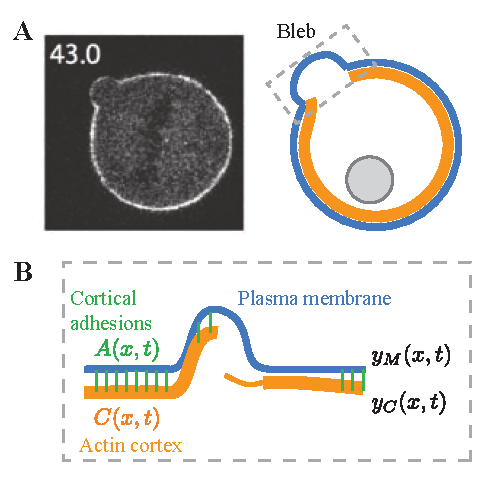
\includegraphics[width=8.5cm]{figs/figSchematic.pdf}
      \caption{(A) Micrograph of a single bleb, induced by laser ablation on the surface of a HeLa cell, 43 seconds after initial formation. Taken from \cite{Biro:2013bk}. (B) Model components. At each location on the surface of the cell $x$, four quantities are represented: The height of the membrane $y_M(x,t)$, the height and thickness of the actin cortex $y_C(x,t)$ and $C(x,t)$ respectively, and the local density of membrane-cortex anchoring proteins, $A(x,t)$. Note that the schematic shows the range of possible model states (e.g., thick or thin cortex, protruding or proximal membrane), while specific predicted dynamics will be determined by simulation.}
      \label{fig::schematic}
   \end{center}
\end{figure}

%%%%%%%%%%%%%%%%%%%%%%%%%%%%%%%%


Our minimal model, summarized schematically in Fig.~\ref{fig::schematic}, consists of four fundamental dynamic variables, as functions of time $t$ and location on the two-dimensional cell surface, parametrized by $(x_1, x_2)$. The actin cortex, has local height described by $Y_C(x_1,x_2,t)$ measured normal to the mean cell surface from its steady-state configuration $Y_C=0$, and thickness $C(x_1,x_2,t)$. The cortical-cytoplasmic actin cytoskeleton can in principle have complicated morphologies that cannot be accounted for by a single location $Y_C$, so we think of $Y_C$ as the weighted average position of maximal cortical actin. Membrane-cortex adhesions are described by density $A(x_1,x_2,t)$ in molecules/ $\text{nm}^2$. Finally, the plasma membrane has local height $Y_M(x_1,x_2,t)$.
%%%%%%%%%%%%%%%%%%%%%%%%%%%%%%%%%%%%%%%%%%%%%%%%%%
%\subsection{Derivation, reduction to one dimensions, and non-dimensionalization}

\subsection{Derivation, and non-dimensionalization}
The dynamics of the actin cortex and  density of adhesions attaching cortex and membrane are governed by
\begin{align}
\dot{C} &= \omega A - \gamma C \label{eq::CDotequation}\\
\dot{A} &=  \frac{\kon\,C}{C_0+C}\; \mbox{exp}\left( - \left(\frac{y-Y_C}{\delta}\right)\right) - \koff A\; \mbox{exp}\left( \frac{k_A (Y_M-Y_C)}{F}\right)\label{eq::ADotequation}
\end{align}

Balance of forces on the cortex is determined by adhesions, which pull the cortex outwards (towards the membrane), and myosin, which contracts, pulling the cortex inwards (towards the cell body):
\begin{align}
0 &= A k_A (Y_M-Y_C) - \sigma_M C Y_C \label{eq::forceBalanceCortex}
\end{align}
Balance of forces on membrane is determined by adhesions, which pull the cortex inwards, and hydrostatic pressure, which pushes the membrane out. 
\begin{align}
0 &= - Ak_A (Y_M-Y_C) + \hat{\Pi}(Y_M^0 - Y_M) + \gamma_M \nabla^2  Y_M \label{eq::forceBalanceMembrane}
\end{align}
Since mechanical equilibration is fast, $Y_M(t)$ and $Y_C(t)$ always evolve to satisfy these equations.


The resulting dimensionless system is:
\begin{align}
\dfrac{dc}{dt}  & =  \Omega a - c\label{eq::nondimc}\\
\epsilon\dfrac{da}{ dt}  & =  \dfrac{c}{1+c} \mbox{exp}\left(-\dfrac{y-y_C}{D}\right) - a \mbox{exp} \left(\dfrac{y-y_C}{F} \right)\label{eq::nondima}\\
0 & = a(y-y_C) - Mcy_C\label{eq::nondimyC}\\
0 & = -a(y - y_C) + P (1-y) + \dfrac{\partial^2 y}{\partial x^2}\label{eq::nondimyM}
\end{align}

%%%%%%%%%%%%%%%%%%%%%%%%%%%%%%%%%%%%%%%%%%%%%%%%%%
\subsection{Formulation as non-local integro-PDE}
%%%%%%%%%%%%%%%%%%%%%%%%%%%%%%%%%%%%%%%%%%%%%%%%%%
Equations ~\ref{eq::nondimc} - ~\ref{eq::nondimyM} can be represented as an integro-PDE. Eq. ~\ref{eq::nondimyM} is a self adjoint. It is very difficult or impossible to find a closed form solution. If we assume a solution exists and has the form $y(x,t) = \int_x h(s,t) ds + r(x,t)$, the we can rewrite the system as:



%%%%%%%%%%%%%%%%%%%%%%%%%%%%%%%%%%%%%%%%%%%%%%%%%%
\subsection{Connections to a larger class of models arising in cell mechanics}
%%%%%%%%%%%%%%%%%%%%%%%%%%%%%%%%%%%%%%%%%%%%%%%%%%
%%%%%%%%%%%%%%%%%%%%%%%%%%%%%%%%%%%%%%%%%%%%%%%%%%
\section{Analysis of ODE system}
%%%%%%%%%%%%%%%%%%%%%%%%%%%%%%%%%%%%%%%%%%%%%%%%%%
While numerical simulation of the full model reveals a range of blebbing behavior, we seek to elucidate how biophysical parameters determine the class of dynamics, specifically whether or not a bleb forms. To this end, we simplify the model by neglecting the tension term in Eq.~\ref{eq::nondimyM}. This transforms the force-balance equations Eq.~\ref{eq::nondimyM}-\ref{eq::nondimyC} into a pair of algebraic equations,
\begin{align}
y &= \frac{(a+cM)P}{a Mc + aP + McP}\label{eq::ODEyM}\\
y_C &= \frac{aP}{a MC + aP + McP}\label{eq::ODEyC},
\end{align}
 These are then substituted into the assembly/disassembly equations, yielding
\begin{align}
\frac{d c}{dt} &= \Omega a - c \label{eq::ODEC}\\
\epsilon \frac{d a}{dt} &= \frac{c}{1+c} \mbox{exp}\left( -\frac{1}{D} \frac{MPc}{a Mc + aP + McP}\right) \notag\\
 &- a\; \mbox{exp}\left( + \frac{1}{F}\frac{MPc}{a Mc + aP + McP}\right) \label{eq::ODEA}
\end{align}
\hspace{10pt}
The model is now a system of two ordinary differential equations (ODEs) amenable to phase plane analysis (Edelstein-Keshet, 1988). 

%%%%%%%%%%%%%%%%%%%%%%%%%%%%%%%%%%%%%%%%%%%%%%%%%%
\subsection{Regimes of behavior at small $\epsilon$}
%%%%%%%%%%%%%%%%%%%%%%%%%%%%%%%%%%%%%%%%%%%%%%%%%%

%%%%%%%%%%%%%%%%%%%%%%%%%%%%%%%%
\begin{figure}[htbp]
  \centering
  \label{fig:phasePlanes}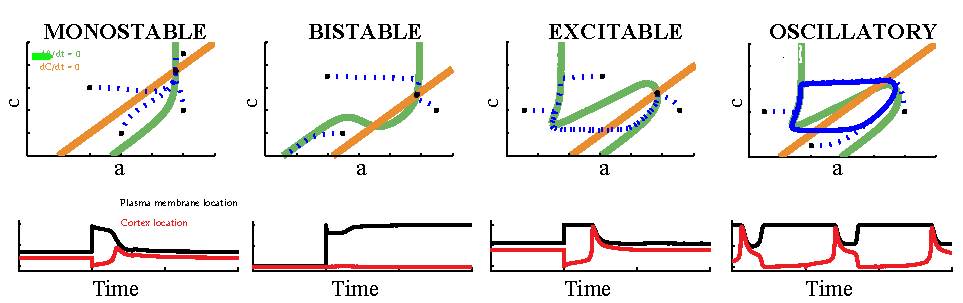
\includegraphics[width=13cm]{figs/figODERegimes.pdf}
  \caption{Phase plane analysis.}
\end{figure}
%%%%%%%%%%%%%%%%%%%%%%%%%%%%%%%%
Figure~\ref{fig:phasePlanes}



%%%%%%%%%%%%%%%%%%%%%%%%%%%%%%%%%%%%%%%%%%%%%%%%%%
\subsection{Bifurcation analysis in $\epsilon$ and $\Omega$}
%%%%%%%%%%%%%%%%%%%%%%%%%%%%%%%%%%%%%%%%%%%%%%%%%%

%%%%%%%%%%%%%%%%%%%%%%%%%%%%%%%%
\begin{figure}[htbp]
  \centering
  \label{fig:2DBifurcation}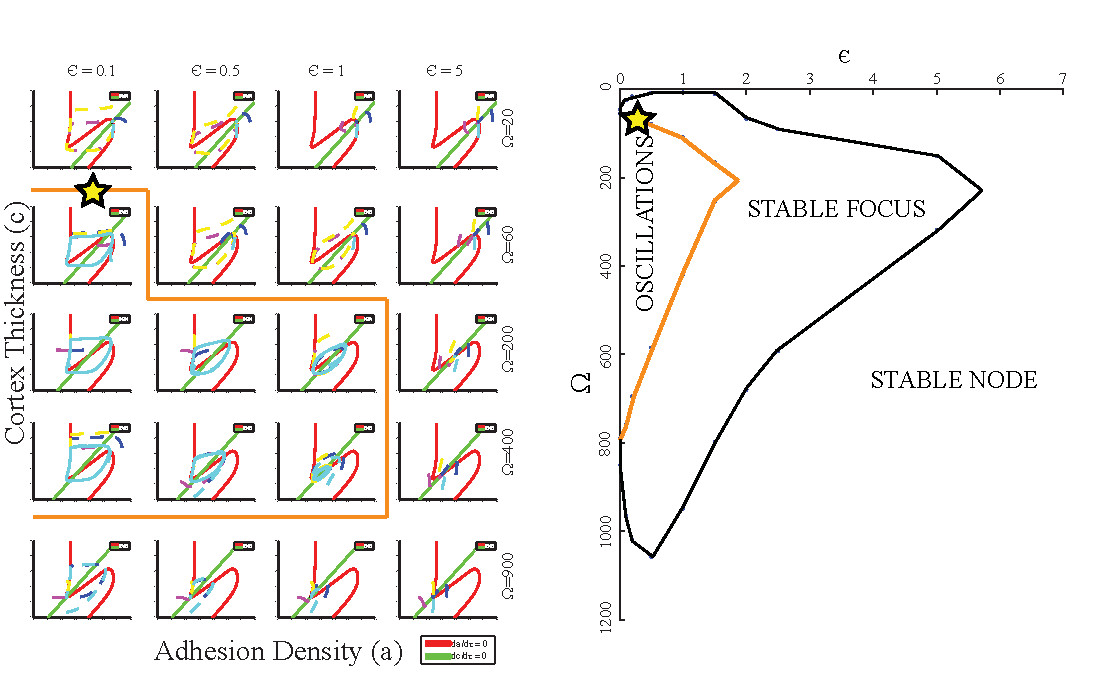
\includegraphics[width=13cm]{figs/fig2DBifurcation.pdf}
  \caption{Bifurcation diagrams.}
\end{figure}
%%%%%%%%%%%%%%%%%%%%%%%%%%%%%%%%
Figure~\ref{fig:2DBifurcation}

%%%%%%%%%%%%%%%%%%%%%%%%%%%%%%%%
\begin{figure}[htbp]
  \centering
  \label{fig:canard}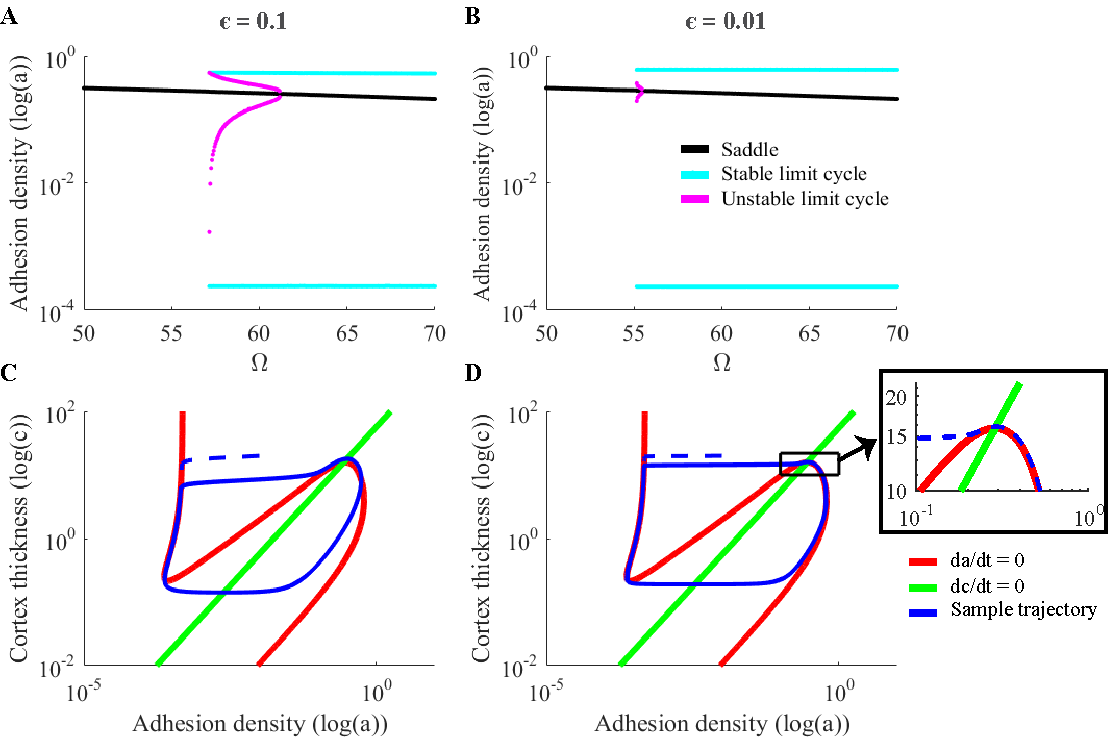
\includegraphics[width=13cm]{figs/figCanard.pdf}
  \caption{Canard explosion.}
\end{figure}
%%%%%%%%%%%%%%%%%%%%%%%%%%%%%%%%
The Duck in Figure~\ref{fig:canard}

%%%%%%%%%%%%%%%%%%%%%%%%%%%%%%%%%%%%%%%%%%%%%%%%%%
\section{Asymptotic analysis of PDE system}
%%%%%%%%%%%%%%%%%%%%%%%%%%%%%%%%%%%%%%%%%%%%%%%%%%

%%%%%%%%%%%%%%%%%%%%%%%%%%%%%%%%%%%%%%%%%%%%%%%%%%
\subsection{Numerical observation of traveling waves}
%%%%%%%%%%%%%%%%%%%%%%%%%%%%%%%%%%%%%%%%%%%%%%%%%%
We are seeking an analog of the Maxwell condition for the bleb model, and similar non-local PDEs. We will make progress toward on this by studying the following systems, from most general (Equations ~\ref{eq::gensystema},~\ref{eq::gensystemy})  to most the most narrow (Equations ~\ref{eq::a_ODE}, ~\ref{eq::gen_ym}).  In the fast timescale, we have $c = c^{ss}$.  The dynamics of excitation are thus only governed by the $a$ equation (Equation ~\ref{eq::nondimA}. We are ultimately interested in a necessary and sufficient traveling wave condition for the general system

\begin{align}
\dfrac{\partial a}{ \partial t}  & =  f(a,y)\label{eq::gensystema}\\
0 & =g \left(a,y,\dfrac{\partial^2 y}{\partial x^2}\right). \label{eq::gensystemy}
\end{align}

Our specific system restricted to the fast timescale is
\begin{align}
\dfrac{\partial a}{ \partial t}  & =  \dfrac{c^{ss}}{1+c^{ss}} \mbox{exp}\left(-\dfrac{y-y_C}{D}\right) - a \mbox{exp} \left(\dfrac{y-y_C}{F} \right)\label{eq::a_ODE}\\
0 & = -a(y - y_C) + P (1-y) + \gamma_M \dfrac{\partial^2 y}{\partial x^2}\label{eq::nondimYm} \\
0 & = a(y-y_C) - Mcy_C\label{eq::nondimyC2}.
\end{align} 
Note that since Eq.~\ref{eq::nondimyC2} is algebraic in $y_C$, we can eliminate it from the system. A narrow version of the system is obtained if we assume the force balance equations are linear in $a$.

\begin{align}
\dfrac{da}{ dt}  & = f_1(y) - a f_2(y)\label{eq::gen_a}\\
0 & = g_1(y) - ag_2(y) +  \dfrac{\partial^2 y}{\partial x^2}\label{eq::gen_ym}
\end{align}
This can be obtained from our system given the following simplifying assumption. Assume that the variable, $y_C$, does not move significantly during excitation, $y_C = y_C^{ss}$, leaving us with a new system of two equations:
\begin{align}
\dfrac{\partial a}{ \partial t}  & =  \dfrac{c^{ss}}{1+c^{ss}} \mbox{exp}\left(-\dfrac{y-y_C^{ss}}{D}\right) - a \mbox{exp} \left(\dfrac{y-y_C^{ss}}{F} \right)\label{eq::a_eq}\\
0 & = -a(y - y_C^{ss}) + P (1-y) + \gamma_M \dfrac{\partial^2 y}{\partial x^2}\label{eq::yM_eq}
\end{align} 
We derive a necessary condition for the system described by Equations ~\ref{eq::a_ODE} and ~\ref{eq::gen_ym} here. 

Numerically, we observe a travelling wave solution to the reduced system described by equations~\ref{eq::a_ODE}, and~\ref{eq::yM_eq} and is shown in Fig.~\ref{fig:numericalTWave}.
%%%%%%%%%%%%%%%%%%%%%%%%%%%%%%%%
\begin{figure}[htbp]
  \centering
  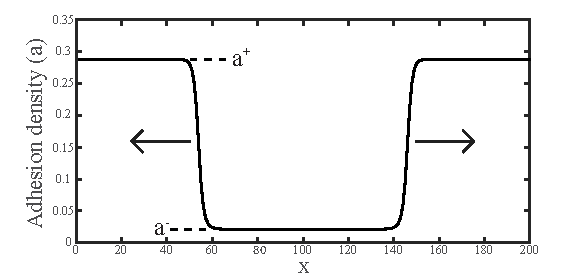
\includegraphics[width=13cm]{figs/figawave.pdf}
  \label{fig:numericalTWave}
  \caption{Numerical observation of traveling wave.}
\end{figure}
%%%%%%%%%%%%%%%%%%%%%%%%%%%%%%%%



%%%%%%%%%%%%%%%%%%%%%%%%%%%%%%%%%%%%%%%%%%%%%%%%%%
 \subsection{Transformation into traveling coordinate $z$ and derivation of a Non-local Maxwell Condition for traveling waves}
%%%%%%%%%%%%%%%%%%%%%%%%%%%%%%%%%%%%%%%%%%%%%%%%%%


%%%%%%%%%%%%%%%%%%%%%%%%%%%%%%%%
\begin{figure}[htbp]
  \centering
  \label{fig:multiscaleRegimes}\includegraphics[width=13cm]{figs/figMultiscaleRegimes.pdf}
  \caption{Decomposition of PDE solution into a traveling wave with regimes in different scales.}
\end{figure}
%%%%%%%%%%%%%%%%%%%%%%%%%%%%%%%%
Figure~\ref{fig:multiscaleRegimes}

%%%%%%%%%%%%%%%%%%%%%%%%%%%%%%%%%%%%%%%%%%%%%%%%%%
%%%%%%%%%%%%%%%%%%%%%%%%%%%%%%%%%%%%%%%%%%%%%%%%%%
We assume, wlog, that Eq.~\ref{eq::gen_a} has two stable roots which we will denote by $(y^{+},a^{+})$ and $ (y^{-},a^{-})$. We will consider only waves traveling from $(y^{+},a^{+})$ to $ (y^{-},a^{-})$ and so movement in this direction will be associated with a positive velocity, $v$. Transform to wave coordinate $z = x-vt$ and~\ref{eq::gen_a} and~\ref{eq::gen_ym} become:
\begin{align}
-v \dfrac{da}{ dz}  & = f_1(y) - a f_2(y)\label{eq::gen_a_z} \\
0 & = g_1(y) - ag_2(y) +  \dfrac{\partial^2 y}{\partial z^2} \label{eq::gen_ym_z}\\ 
\end{align}

We can use Eq. ~\ref{eq::gen_ym_z} to solve for $a$:
\begin{flalign}
 a = \dfrac{1}{g_2(y)} \left( g_1(y) + \dfrac{\partial^2 y}{\partial z^2} \right)
\end{flalign}
Then it follows that:
\begin{equation}\Rightarrow  -v \dfrac{\partial a}{ \partial z}   =  f_1(y)  -  \dfrac{g_1(y)}{g_2(y)}f_2(y) - \dfrac{f_2(y)}{g_2(y)} \dfrac{\partial^2 y}{\partial z^2}
\end{equation}
Multiply by $ \dfrac{g_2(y)}{f_2(y)} $,
\begin{equation}\Rightarrow   -v \dfrac{\partial a}{ \partial z} \dfrac{g_2(y)}{f_2(y)}   =  f_1(y)\dfrac{g_2(y)}{f_2(y)}  -  g_1(y) -  \dfrac{\partial^2 y}{\partial z^2}
\end{equation}
Multiply by $\dfrac{\partial y}{\partial z}$,
\begin{equation}\Rightarrow  -v \dfrac{\partial a}{ \partial z} \dfrac{g_2(y)}{f_2(y)} \dfrac{\partial y}{\partial z}   =  \left( f_1(y)\dfrac{g_2(y)}{f_2(y)}  -  g_1(y) -  \dfrac{\partial^2 y}{\partial z^2} \right)  \dfrac{\partial y}{\partial z}
\end{equation}
Integrate over $z$, 
\begin{equation}
\Rightarrow  \int_ {- \infty}^{\infty}  -v \dfrac{\partial a}{ \partial z} \dfrac{g_2(y)}{f_2(y)} \dfrac{\partial y}{\partial z} dz = \int_ {- \infty}^{\infty} \left( f_1(y)\dfrac{g_2(y)}{f_2(y)}  -  g_1(y) -  \dfrac{\partial^2 y}{\partial z^2} \right)  \dfrac{\partial y}{\partial z} dz
\end{equation}
Change variables on RHS,   
\begin{align}
\Rightarrow -v  \int_ {- \infty}^{\infty}  \dfrac{\partial a}{ \partial z} \dfrac{g_2(y)}{f_2(y)} \dfrac{\partial y}{\partial z} dz &= \int_ {y^{-}}^{y^{+}} \left( f_1(y)\dfrac{g_2(y)}{f_2(y)}  -  g_1(y) -  \dfrac{\partial^2 y}{\partial z^2} \right)  dy \\
\Rightarrow  -v  \int_ {- \infty}^{\infty}  \dfrac{\partial a}{ \partial z} \dfrac{g_2(y)}{f_2(y)} \dfrac{\partial y}{\partial z} dz &= \int_ {y^{-}}^{y^{+}} \left( f_1(y)\dfrac{g_2(y)}{f_2(y)}  -  g_1(y)\right) dy -  \cancelto{0}{\int_ {y^{-}}^{y^{+}}  \dfrac{\partial^2 y}{\partial z^2}   dy}\\
\Rightarrow -v  \int_ {- \infty}^{\infty}  \dfrac{\partial a}{ \partial z} \dfrac{g_2(y)}{f_2(y)} \dfrac{\partial y}{\partial z} dz &= \int_ {y^{-}}^{y^{+}} \left( f_1(y)\dfrac{g_2(y)}{f_2(y)}  -  g_1(y)\right) dy \label{eq::NLMC}\\
\end{align}

The Non-local Maxwell Condition Number is defined by the RHS of Eq.~\ref{eq::NLMC}. In our specific case,
\begin{align}
f_1(y) &=  \dfrac{c^{ss}}{1+c^{ss}} \mbox{exp}\left(-\dfrac{y-y_C^{ss}}{D}\right),\\
f_2(y) &= \mbox{exp} \left(\dfrac{y-y_C^{ss}}{F} \right),\\
g_1(y) &=  P (1-y), \\
 g_2(y) &= (y - y_C^{ss}).
\end{align}
Therefore, 
\begin{multline}
-v  \int_ {- \infty}^{\infty}  \dfrac{\partial a}{ \partial z} \dfrac{(y - y_C^{ss})}{ \mbox{exp} \left(\dfrac{y-y_C^{ss}}{F} \right)} \dfrac{\partial y}{\partial z} dz \\
= \int_ {y^{-}}^{y^{+}} \left( \dfrac{c^{ss}}{1+c^{ss}} \mbox{exp}\left(-\dfrac{y-y_C^{ss}}{D}\right) \dfrac{(y - y_C^{ss})}{ \mbox{exp} \left(\dfrac{y-y_C^{ss}}{F} \right)}  -   P (1-y) \right) dy
\end{multline}
\begin{multline}
\implies -v  \int_ {- \infty}^{\infty}  \dfrac{\partial a}{ \partial z}\dfrac{\partial y}{\partial z} \mbox{exp} \left(-\dfrac{y-y_C^{ss}}{F} \right)(y - y_C^{ss}) dz \\
= \int_ {y^{-}}^{y^{+}}  \left( \dfrac{c^{ss}}{1+c^{ss}} \mbox{exp}\left( -\left( \dfrac{1}{D} + \dfrac{1}{F} \right) (y-y_C^{ss})\right)  -   P (1-y) \right) dy
\end{multline}
We also note that in our specific case $y^- > y^+$ and so it makes sense to integrate from $y^+$ to $ y^-$.
\begin{align*}
\Rightarrow & -v  \int_ {- \infty}^{\infty}  \dfrac{\partial a}{ \partial z}\dfrac{\partial y}{\partial z} \mbox{exp} \left(-\dfrac{y-y_C^{ss}}{F} \right)(y - y_C^{ss}) dz\\
& \hspace{2cm}= - \int_ {y^{+}}^{y^{-}}  \left( \dfrac{c^{ss}}{1+c^{ss}} \mbox{exp}\left( -\left( \dfrac{1}{D} + \dfrac{1}{F} \right) (y-y_C^{ss})\right)  -   P (1-y) \right) dy
\end{align*}
Our Non-Local Maxwell condition Number is:
\begin{align}
NLMC &= -\int_ {y^{+}}^{y^{-}}  \left( \dfrac{c^{ss}}{1+c^{ss}} \mbox{exp}\left( -\left( \dfrac{1}{D} + \dfrac{1}{F} \right) (y-y_C^{ss})\right)  -   P (1-y) \right) dy \\
 &= \dfrac{c^{ss}}{1+c^{ss}}  \mbox{exp}\left( +\left( \dfrac{1}{D} + \dfrac{1}{F} \right)y_C^{ss}  \right) \left( y^--y^+ \right) + P\left( 1 - \frac{1}{2}\left( \left(y^+\right)^2-\left(y^-\right)^2\right)\right)
\end{align}
The integral on the LHS is of determined sign (-).  Therefore, the Nonlocal Maxwell Condition is:
\begin{align*}
& NLMC >0 \Rightarrow v \text{ exists, travelling solution}\\
& NLMC <0 \Rightarrow v \text{ does not exist, stationary solution}
\end{align*}
Note that only the second line (necessity) is shown here. The first line (sufficiency) is supported by numerical evidence below.

After we hold $c$ and $y_C$ constant, we end up with a single PDE. Dropping the spatial term, and analyzing the single ODE we find that the ODE is can be monostable low, monostable high, in which case there is a single steady state solution or it can be bistable. See Fig.~\ref{fig::phaseline} for a plot of the single ODE in the various regimes. 

The non-local Maxwell condition is equal to $0$ in both of the monostable regimes (because $y^- = y^+$), but can be negative or positive in the bistable regime. Returning to the PDE, we don't expect travelling solutions to arise from a monostable regime, but we wish to see for which region of the bistable regime the non-local Maxwell condition predicts travelling solutions. By varying two parameters continuously we can determine these regions. This is shown in Fig.~\ref{fig::NLMC}(A). Here the parameters varied are $\Omega$ which is not present in the single PDE but changes are reflected in $c^{ss}$, and $F$. We plan to create identical plots using other pairs of parameters. The regions shown in Fig.~\ref{fig::NLMC} (A) match up well with the numerical solutions of the PDE as depicted in Eq.~\ref{fig::NLMC} (B), which shows the velocity of the travelling wave solution ($=0$ for a stationary solution).

%%%%%%%%%%%%%%%%%%%%%%%%%%%%%%%%
\begin{figure}[htbp]
  \centering
  \label{fig:NLMC}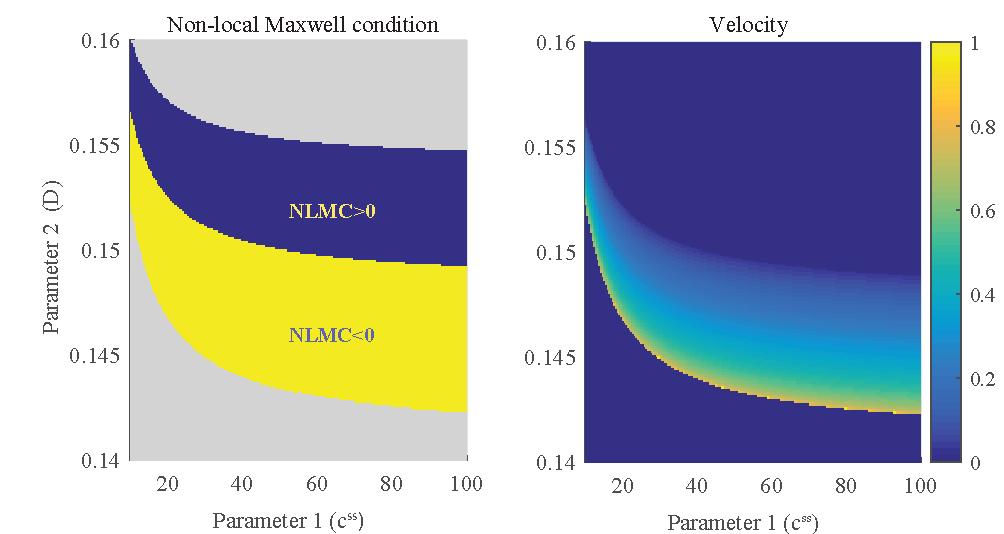
\includegraphics[width=13cm]{figs/figNLMC.pdf}
  \caption{Nonlocal Maxwell condition demonstrating emergence of traveling waves.}
\end{figure}
%%%%%%%%%%%%%%%%%%%%%%%%%%%%%%%%
\ref{fig:NLMC}



\appendix
%\section{An example appendix} 
%\lipsum[71]

\section*{Acknowledgments}
We would like to acknowledge .

\bibliographystyle{siamplain}
\bibliography{references}
\end{document}
